\documentclass[10pt,twocolumn,letterpaper]{article}

\usepackage{cvpr}
\usepackage{times}
\usepackage{epsfig}
\usepackage{graphicx}
\usepackage{amsmath}
\usepackage{amssymb}
\usepackage{natbib}
\usepackage{float}


% Include other packages here, before hyperref.

% If you comment hyperref and then uncomment it, you should delete
% egpaper.aux before re-running latex.  (Or just hit 'q' on the first latex
% run, let it finish, and you should be clear).
\usepackage[breaklinks=true,bookmarks=false]{hyperref}

\cvprfinalcopy % *** Uncomment this line for the final submission

\def\cvprPaperID{****} % *** Enter the CVPR Paper ID here
\def\httilde{\mbox{\tt\raisebox{-.5ex}{\symbol{126}}}}

% Pages are numbered in submission mode, and unnumbered in camera-ready
%\ifcvprfinal\pagestyle{empty}\fi
\setcounter{page}{1}
\begin{document}

%%%%%%%%% TITLE
\title{Comparing Pixel Inputs and Structured Inputs in Reinforcement Learning with Self-Play}

\author{Brendon Go\\
Stanford University\\
{\tt\small go@cs.stanford.edu}
% For a paper whose authors are all at the same institution,
% omit the following lines up until the closing ``}''.
% Additional authors and addresses can be added with ``\and'',
% just like the second author.
% To save space, use either the email address or home page, not both
\and
Evan Liu\\
Stanford University\\
{\tt\small evanliu@cs.stanford.edu}
}

\maketitle
%\thispagestyle{empty}

\section{Introduction}

In the Reinforcement Learning (RL) paradigm, agents learn to perform complex
tasks through trial-and-error. The agents take certain actions and observe their
consequences (reward) -- learning to prefer actions that lead to positive
consequences.  This paradigm has shown great promise in disparate
applications, ranging from dialogue generation \citep{dialogue2016}, to game
playing \citep{mnih2015human}, to robotics \citep{robotics2016}.

Recent RL methods have achieved superhuman performance on Atari 2600 games
\citep{bellemare2013arcade}. These methods receive as input the raw pixels that
appear on the game screen, and output actions (e.g. moving left or right),
learning to find action sequences that maximize the game score. Traditional
wisdom posits that the task would be easier if the input were structured (e.g.
the positions of the character and enemies in the game) rather than pixels,
because with pixel inputs, the pixels must first be processed to extract this
structured information. However, surprisingly, on a version of the Atari 2600
games, where the inputs to the RL agent are the game memory (which include
information like the coordinates of the avatar), current RL methods perform
poorly, far worse than on the pixel version \citep{atariRAM}.

We investigate this phenomenon on games outside of Atari to determine
if the poor performance is an artifact of the structure of Atari games or if
there is a deeper reason. In particular, we focus on a favorite game from the
90s, Slime Volleyball, where the goal of the game is to hit a ball over a net
onto the opponent's side of the game. Players win points when the ball hits the
ground on the opponent's side of the net. We apply deep RL methods to
this game with two types of inputs: the pixels of the game screen, and the
variables used to generate the game, and compare the performance of these
algorithms on different types of inputs. Success on this project will hopefully
lend greater insight into why Atari on RAM states fails, possibly leading to
novel RL algorithms or insights about the pixel states. In the process, we
also investigate into self-play methods in RL, \citep{silver2016mastering} which
have shown grown success in learning to solve complex tasks.

\section{Task}

We operate in a Markov Decision Process (MDP), consisting of the set of
possible states $\mathcal{S}$, the set of possible actions $\mathcal{A}$, the
reward dynamics $\mathcal{R}: \mathcal{S} \times \mathcal{A} \to \mathbb{R}$,
describing what rewards the agent receives when it plays a certain action in a
certain state, the environment dynamics $P: \mathcal{S} \times \mathcal{A}
\times \mathcal{S} \to \mathbb{R}$ describing the probability of transitioning
to a new state from the current state after taking an action, and a discount
factor $\gamma$. States $s \in \mathcal{S}$ are assumed to have the
Markov-property: the current state contains all of the necessary information to make
decisions. The goal is to learn a policy $\pi$ that maps a state to the action
to take in that state that maximizes the expected discounted reward.

In contrast to the traditional single-agent RL setup, which includes only a
single RL agent, our setting contains two RL agents that play against each
other. Notably, from the point of view of the first agent, the environment
dynamics function $P$ encodes the policy of the other agent -- when the other
agent's policy changes, the environment dynamics model also change. This means
that the environment dynamics model is non-stationary if both agents are
learning, and that the environment dynamics model differs between the points
of views of the first and second agents. This introduces additional technical
challenges addressed in Section \ref{technical}.

\subsection{Slime Volleyball}


\begin{figure}[h]
\center
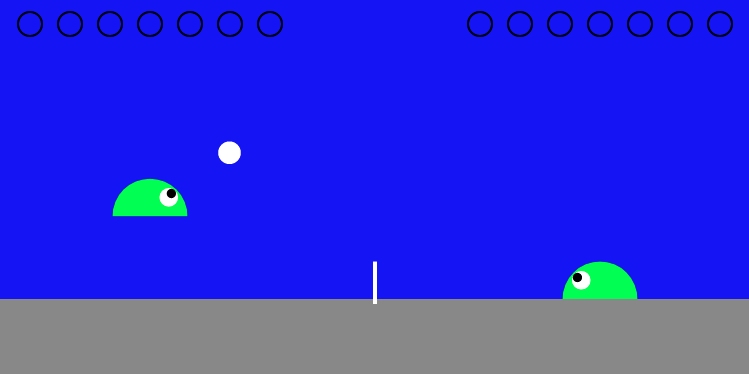
\includegraphics[width=\columnwidth]{SlimeVolleyBall}
\caption{
Player 1 Serving the ball over the net in Slime Volleyball
}\label{fig:slime}
\end{figure}


In Slime Volleyball, there are two agents, on either set of a volleyball net.
On each point, the agents attempt to hit the volleyball over the net to the
opponent's side. If the ball hits the ground on the opponent's side, the agent
wins the point and receives reward $+1$. If the ball hits the ground on the
agent's side, the agent receives reward $-1$, and $0$ reward while the point
is still in play. The game terminates after either agent wins $7$ points. To
hit the ball, the agent can take actions of moving left, right, or jumping.
The ball bounces off the agent's head when the agent collides with the ball.
Notably, agents can jump as many times as they wish, and can also jump over
the net to the opponent's side of the net.

We have modified an HTML5 implementation of Slime Volleyball, to use
as a browser-based simulation environment. Following \citep{shi2017world}, we use
Selenium to send actions to the browser simulation environment and receive
responses to update the agents. The browser simulation environment is
configured to run in two modes: pixel states and structured states. In the
pixel state mode, the agent receives as input the screenshot of the screen. In
structured state mode, the agent receives as input a structured list
consisting of the $(x, y)$ coordinates and velocity of the agent, the
opponent, and the ball, as well as the current score. Notably, the states are
configured such that reflecting the pixel or structured state for the first
agent over the x-axis results in the state of the second agent. This enables
us to maintain a single model act for both agents.

\subsection{Goal}

Our goal is to compare the performance of agents that use pixel state vs.
agents that use structured state. Concretely, we seek to answer the following
questions:

\paragraph{Training Speed and Asymptotic Performance without Self-Play.} In
Atari, we are surprised to find that models that use structured inputs far
underperform models that use pixel inputs. This may be due to some of the
intuitions that make SVMs work -- pixel inputs effectively project the
structured inputs to a much higher dimension to perform computation. We seek
to understand if this phenomenon holds in Slime Volleyball. To evaluate this,
we train a pixel-input agent and a structured-input agent against a
fixed random opponent. This attempts to isolate effects of self-play vs. the
effects of differing inputs. We report on sample efficiency (number of samples
to required to learn) and asymptotic performance (average episode reward after
training converges).

\paragraph{Performance with Self-Play.} We further are interested in the
effects of self-play combined with differing inputs. To evaluate this, we
propose to play an agent using pixel-inputs against an agent using
structured-inputs. We will use alternating optimization on each agent and
report on sample efficiency and asymptotic performance.

\paragraph{Comparison with Human Play.} Finally, we also want to compare our
models against humans. We propose not to directly optimize against human play,
but learn models via self-play. After many rounds of self-play, we will play
the trained models against humans and report the asymptotic performance.
Notably, humans might use strategies that are not seen during self-play.
Results could be particularly interesting if the models perform well even
against these novel strategies.

\section{Technical Approach}
\label{technical}
\subsection{Deep Q-Learning}

We implement the policies for each agent as Deep Q-Networks \citep{nature2013}.
In Deep Q-Learning, a value function $Q(s, a)$ is learned that estimates the
discounted reward to go that the agent will receive for playing action $a$ in
state $s$ and continuing to follow its current policy. The learned $Q$ function
encodes a policy, which at each state $s$ plays the action $a = argmax_{a \in
\mathcal{A}}Q(s, a)$. Our $Q$ functions are implemented as neural networks. For
structured state inputs, the network consists of several multi-layer perceptrons
(MLP). For pixel state inputs, the network consists of several convolutional
layers, followed by a MLP. The encoded policy can be made non-greedy by
following an $\epsilon$-greedy policy, which greedily chooses the best action
$a$ according to $Q$ with probability $1 - \epsilon$ and choosing a random
action with probability $\epsilon$. We utilize an $\epsilon$-greedy policy with
an $\epsilon$ that anneals to $0$ during training to ensure that the policy
adequately explores the state and action spaces.

The $Q$ function is updated by taking gradient steps to minimize the
following loss function, which corresponds to the Bellman update:

\begin{equation}
  ||Q(s, a) - (r + \gamma \max_{a' \in \mathcal{A}}Q(s', a'))||^2_2
\end{equation}

\noindent updated on a single experience $(s, a, r, s')$. This experience
corresponds to the an observation of taking action $a$ in state $s$, resulting
in the new state $s'$ and reward $r$. $\gamma \in [0, 1]$ is the discount
factor, which controls how valuable it is to get reward in the future.
Notably, the DQN algorithm is off-policy, meaning that these $(s, a, r, s')$
experiences may be collected from following any policy, so long as the policy
plays every action with a non-zero probability.

Following \citep{nature2013}, we make use of experience replay for learning $Q$. The
agent follows an the $\epsilon$-greedy policy recording all experiences $(s, a,
r, s')$ in a fixed-size replay buffer. Periodically during training, a batch
of experiences is sampled and the above loss function is minimized on the
batch of experiences. Experience replay enables updates with
removed temporal correlations. In addition, Q-learning requires many updates
to ensure that later $Q$ values propagate backwards to earlier $Q$ values and
experience replay helps propagation happen. Finally, experience replay also
helps with sample efficiency, since each experience may be updated on many
times.

\paragraph{Double Deep Q-Networks}
In addition, to help stabilize the DQN updates, we make usage of double deep
q-networks \citep{doubleDQN}. In the original formulation of DQN, the
$\max_{a' \in \mathcal{A}}Q(s', a')$ term in the loss can be overly optimistic
(too large) from initialization and stochasticity, pushing the $Q$ values to
be higher than they should be. In order to avoid this issue, we maintain two
$Q(s, a)$ functions, one parametrized by $\theta$, $Q(s, a; \theta)$ and
another parametrized by $\theta'$, $Q(s, a; \theta')$. In the new update, we
take the maximum action over one of the networks, but use the value from the
other network:

\begin{equation}
  ||Q(s, a) - (r + \gamma Q(s', arg\max_{a' \in \mathcal{A}}Q(s', a'; \theta'); \theta))||^2_2
\end{equation}

\noindent This new update helps avoid over-estimating the max $Q$ value.

\subsection{Self-Play}

As previously mentioned, when both agents are updating, the environment
dynamics appear non-stationary. Notably, in multi-agent systems, independent
Q-Learning \citep{tan1993multi}, where each agent maintains its own $Q$
function fails precisely because of the non-stationaryness. To avoid this
problem, during self-play, we initialize two copies of the same policy (the
$Q$ network), which we term the leader and the challenger. During training, we
fix the parameters of the leader, while the challenger trains against the
leader using the previously described deep q-learning algorithms.
Periodically, to ensure that the leader is also training, we clear the replay
buffer and set the leader's parameters equal to the challenger's updated
parameters. We are required to throw away the replay buffer when we change the
leader because the replay buffer encodes information about the environment
dynamics. When the leader changes, the environment dynamics effectively
change, so the information in the replay buffer is now useless.

\paragraph{Generalization}

When the agent is trained using self-play exactly as above, it faces issues of
generalization against unseen opponents. Ideally, after self-play, we'd like
for our agent to perform well against all other types of opponents, not just
opponents that play like itself. Drawing a connection to supervised learning,
there is a distribution of all agents for the game. During training, we sample
agents from this distribution (in our case, our samples are exactly the copies
of the agent being trained) and training against those agents. During test
time, we hope to perform well against other agents drawn from the distribution
that we never saw during training time. In the above algorithm, the agent only
sees very few types of other opponents, and so when playing against new unseen
opponents, it performs poorly.

To remedy this issue, we keep track of the best $k$ parameters and train
against $k$ leaders. At the beginning of a training round, $k$ leaders and $k$
challengers are initialized with the best $k$ parameters (or randomly
initialized if $k$ parameter sets have not yet been created). During training,
we again fix the parameters of the leaders and update the parameters of the
challengers through updates with the replay buffer. During each episode, we
randomly sample one leader and one follower. Periodically, we save the
parameters of the challengers and add them to the list of previous parameters.
After a fixed number of steps, we select the top $k$ parameters by doing a
round-robin evaluation of parameters against each other, discarding the rest
of the parameters. To begin the next round, we clear the replay buffer and
reinitialize the leaders and challengers with the top $k$ parameters. In our
experiments, we use $k = 5$.

By training against many leaders and selecting the parameters that perform
best against all the other parameters, we prevent the agent from overfitting
to playing against itself. Empirically, we observed that when setting $k = 1$,
the agent performed far worse against unseen opponents than when $k = 5$.
Additionally, using multiple challengers that share a replay buffer can be
viewed as a form of bootstrapped DQN \citep{osband2016deep}. Although the
multiple challengers do not share parameters, by allowing each challenger to
update on the experiences of other challengers, we achieve better exploration.
In contrast to just $\epsilon$-greedy approaches, which make locally
non-greedy decisions, by observing the other challengers, we achieve
temporally extended exploration, where we can explore with an entirely
different policy. This leads to faster training and improved asymptotic
performance.

\section{Results}

\subsection{Experimental Details}
We implemented both the pixel-state model and the structured-state model in
PyTorch \citep{paszke2017automatic}. As inputs to the pixel-state model, we
preprocess the pixel values of the original $750$ by $375$ gamescreen and
downsample to a $84$ by $84$ pixel grid. In order to capture velocity
information, we stack the past $4$ frames. We feed in the grayscale pixel
values of the stacked frames to the pixel-state model. The pixel-state network
consists of three convolutional layers followed by two fully connected layers,
following \citep{nature2013}. The first layer contains $32$ filters, a square kernel
of size $8$, and stride $4$. The second layer contains $64$ filters, a square
kernel of size $4$ and stride $2$. The third layer contains $64$ filters, a
square kernel of size $3$ and stride $1$. The fourth layer is a fully
connected layer that is $6400$ by $512$. The output layer is a fully connected
layer that is $512$ by $6$, which is the number of actions.

As inputs to the structured-state model, we normalize the structured states to
be between $0$ and $1$. We then pass it through four fully connected layers
with output sizes $128$, $128$, $128$, and $6$ respectively.

Unless otherwise mentioned, we train each agent for $10$ rounds of self-play,
each round consisting of $390000$ frames, saving parameters every $130000$
steps. We start taking gradient steps from the replay buffer after $50000$
frames and take a gradient step every $4$ steps on a batch size of $32$
experiences. Both policies use an $\epsilon$-greedy exploration strategy, with
$\epsilon$ starting at $1$ and annealing to $0.01$ over the $390000$ frames.
We use the Adam optimizer \citep{kingma2014adam} with learning rate $0.00025$.
We use a discount factor $\gamma$ of $0.99$.

\subsection{Sample Complexity and Asymptotic Performance of Pixels vs
Structured States}
To evaluate the sample complexity differences and the asymptotic performance
differences of the pixel-state agent and the structured-state agent, we train
both agents against a fixed simple hand-coded agent. We train both agents
until their policies have converged (on an $\epsilon$-greedy schedule
annealing from $1$ to $0$ in $1000000$ frames). After training, the
pixel-state agent wins by an average of $6.92$ points per episode and the
structured-state agent wins by an average of $6.84$ points per episode,
averaged over $1000$ episodes. This suggests that the asymptotic performances
of both models is similar. However, the structured-state agent trains to
convergence in approximately $3000000$ frames, while the pixel-state agent
takes approximately $8000000$ frames to converge. This is not so surprising,
because the structured-state agent has far fewer parameters than the
pixel-state agent, and the structured-state agent does not need to extract as
much information from the state as the pixel-state agent.

\subsection{Generalization Against Unseen Opponents}
We further evaluate the trained pixel-state agents and structured-state agents
against new opponents that were never seen during training to evaluate their
ability to generalize. To do this, we evaluate against a human, a very strong
hand-coded agent (about 200 lines of code designed to play well and make
tricky shots), and against the agent using the other type of state
(pixel-state vs. structured-state) and report the score of the agent on the
left minus the score of the agent on the right, averaged over $1000$ episodes.
The results of these experiments are summarized in \ref{fig:results}.

\begin{figure}[H]
\center
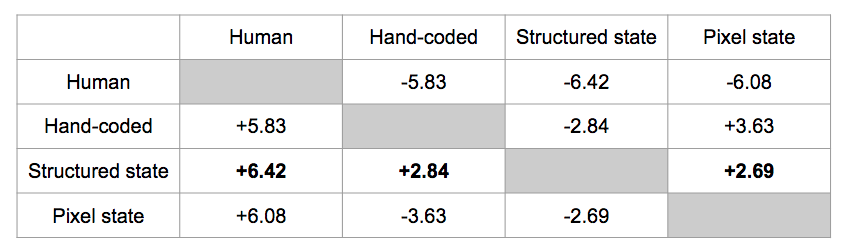
\includegraphics[width=\columnwidth]{results}
\caption{
Score of Left Agent - Score of Top Agent Averaged over 1000 games
}\label{fig:results}
\end{figure}

Interestingly, the pixel-state and structured-state agents consistently beat the
human, even though the human plays very differently from either of them. This
suggests that our self-play algorithm successfully trains agents that
generalize. In addition, the structured-state agent beats the hand-coded
agent, even though the hand-coded agent is quite strong (it consistently beats
the human). The pixel-state agent also performs reasonably well against the
hand-coded agent, although it does lose. The pixel-state agent performs well
but not as well as the structured-state agent, suggesting that learning from
structured-state is really better than learning from the pixel-state. This
suggests that the results on Atari may be due to the extraneous information in
the RAM states, rather than due to the structured vs. unstructured states.
Further analysis on Atari is required to definitively determine what causes
RAM state agents to perform worse than pixel state agents.

Notably, the pixel-state agent may perform less well than the structured-state
agent due to learning speed. As shown in the previous experiments, the
pixel-state agent requires more samples to learn than the structured-state
agent, but in these experiments, they were trained for the same number of
steps due to limited computation. However, it is still an important result to
note that structured-state agents can learn more quickly.

Videos of our agents in action are available in the supplementary materials.

\subsection{Analysis}

\begin{figure}[H]
\center
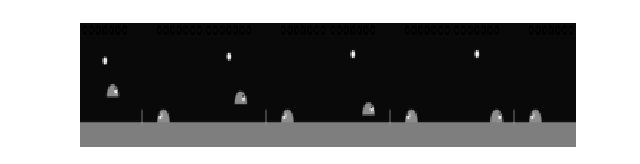
\includegraphics[width=\columnwidth]{preprocess}
\caption{
Visualizing Hidden States: Preprocessed Pixel State
}\label{fig:preprocess}
\end{figure}

\begin{figure}[H]
\center
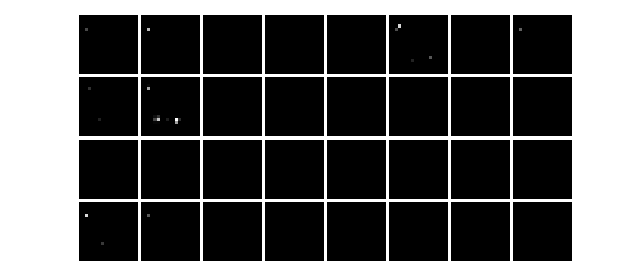
\includegraphics[width=\columnwidth]{layer1}
\caption{
Visualizing Hidden States: First Hidden Layer
}\label{fig:layer1}
\end{figure}

\begin{figure}[H]
\center
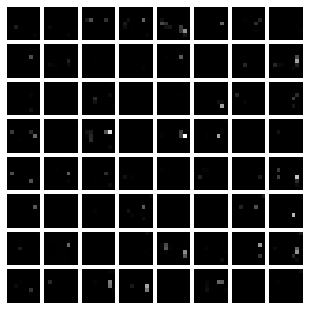
\includegraphics[width=\columnwidth]{layer2}
\caption{
Visualizing Hidden States: Second Hidden Layer
}\label{fig:layer2}
\end{figure}

\begin{figure}[H]
\center
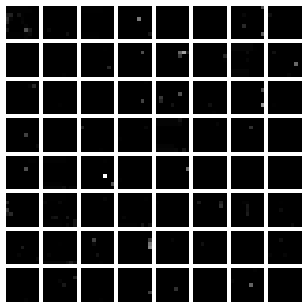
\includegraphics[width=\columnwidth]{layer3}
\caption{
Visualizing Hidden States: Third Hidden Layer
}\label{fig:layer3}
\end{figure}

We can visualize what our CNN is doing by feeding a state into the CNN and
displaying the output of each layer as a set of images. Figures \ref{fig:preprocess}
to \ref{fig:layer3} show an example of this visualization. We can see that
the first hidden layer has some filters that pick out the locations of the ball,
our own slime, our enemy slime, or some combination of these three. The second
and third hidden layer somehow encode some other higher level features we
suspect the streak like patterns could perhaps be encoding the velocities.

{\small
\bibliographystyle{unsrtnat}
\bibliography{egbib}
}

\end{document}
